\documentclass[border=20pt]{standalone}
\renewcommand\familydefault{\sfdefault} % Default family: serif
\usepackage{tikz}
\usetikzlibrary{calc}
\usetikzlibrary{shapes.geometric}
\usetikzlibrary{arrows.meta,arrows}
\usetikzlibrary{positioning}
\tikzset{
  initial/.style={circle, fill},
  decision/.style={diamond, black, draw},
  action/.style={rectangle, draw, rounded corners},
  arrow/.style={draw, -{Latex[length=3mm]}, thick}
  }
\begin{document}
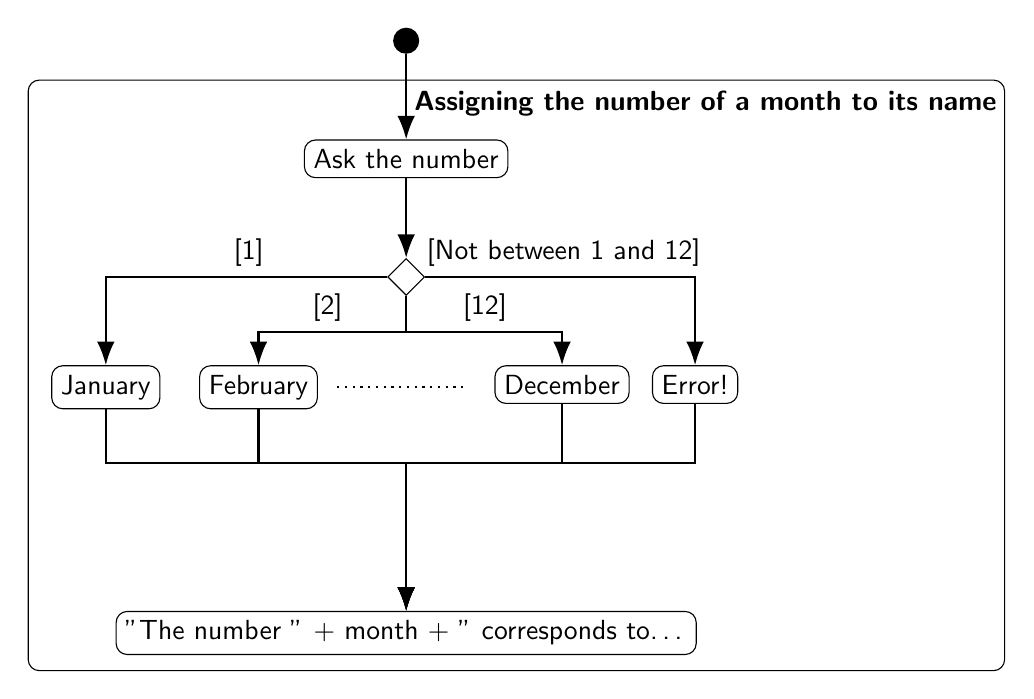
\begin{tikzpicture}[node distance=1.5cm]
	% Frame
	\draw [rounded corners] (-4.8,-1.5) rectangle (7.6, -9);
	\node (title) at (3.8, -1.8) {\textbf{Assigning the number of a month to its name}};

	% Nodes
	\node[initial] (initial) at (0,-1) {};
	\node[action, below of = initial] (ask)  {Ask the number};
	\node[decision, below of= ask] (decision1)  {};
	\node[action, below left = 1cm and 3cm of decision1] (jan) {January};
	\node[action, below left = 1cm and 1cm of decision1] (feb) {February};
	\node[action, below right = 1cm and 1cm of decision1] (dec) {December};
	\node[action, below right = 1cm and 3cm of decision1] (error) {Error!};
	\node[action, below = 4cm of decision1] (exit) {"The number " + month + " corresponds to…};


	% Arrow
	\draw [arrow] (initial) -- (ask);
	\draw [arrow] (ask) -- (decision1);
	\draw [arrow] (decision1) -- node[above, pos=1pt]{[1]} ++(-2cm, 0) -| (jan);
	\draw [arrow] (decision1) -- ++(0, -.7cm) -- node[above, pos=1pt]{[2]} ++(-1cm, 0cm) -| (feb);
	\draw [arrow] (decision1) -- ++(0, -.7cm) -- node[above, pos=1pt]{[12]} ++(1cm, 0cm) -| (dec);
	\draw [arrow] (decision1) -- node[above, pos=1pt]{[Not between 1 and 12]} ++(2cm, 0) -| (error);

	\draw [arrow] (jan)  -- ++(0cm, -.96cm) -| (exit);
	\draw [arrow] (feb)  -- ++(0cm, -.96cm) -| (exit);
	\draw [arrow] (dec)  -- ++(0cm, -1cm) -| (exit);
	\draw [arrow] (error)  -- ++(0cm, -1cm) -| (exit);

%	\draw [arrow] (decision2) -- node[above, pos=1pt]{[Quiz]} ++(-2cm, 0) -| (quiz);
%	\draw [arrow] (decision2) -- node[above, pos=.7pt]{[No quiz]} ++(2cm, 0) -| (class);

	% Etc.
	\draw[dotted, thick] ($ (feb)+(1,0)$) -- ++(1.6, 0);
\end{tikzpicture}
\end{document}

